\documentclass[11pt]{article}
\usepackage[a4paper,margin=1in]{geometry}
\usepackage{amsmath,amssymb,amsfonts}
\usepackage{graphicx}
\usepackage{booktabs}
\usepackage{siunitx}
\usepackage{xcolor}
\usepackage{enumitem}
\usepackage[colorlinks=true,linkcolor=blue,citecolor=blue,urlcolor=blue]{hyperref}
\usepackage{caption}
\captionsetup{font=small,labelfont=bf}

\newcommand{\eps}{\varepsilon}
\newcommand{\vecr}{\mathbf{r}}
\newcommand{\veck}{\mathbf{k}}
\newcommand{\vecE}{\mathbf{E}}
\newcommand{\vecj}{\mathbf{j}}
\newcommand{\Om}{\hat{\boldsymbol{\Omega}}}
\newcommand{\gradr}{\nabla_{\!\vecr}}
\newcommand{\honest}[1]{\par\medskip\noindent{\setlength{\fboxsep}{7pt}%
\colorbox{yellow!22}{\begin{minipage}{\dimexpr\linewidth-2\fboxsep\relax}%
\small\textbf{Reconstruction note.} #1\end{minipage}}}\par\medskip}
\newcommand{\fix}[1]{\textcolor{green!45!black}{\small[\textbf{Rev.4:} #1]}}

\title{\textbf{Derivation and Numerical Reproduction of\\
Liang, Goldsman, Mayergoyz \& Oldiges (1997):\\
2-D MOSFET Modeling by Self-Consistent Solution of the\\
Boltzmann, Poisson, and Hole-Continuity Equations}\\[4pt]
\large\textit{Part~I --- Method derivation and documented solver foundation}\\
\normalsize\textbf{Revision~4} (third-audit response)}
\author{Reproduction study \quad\small(code commit \texttt{e71677b}; Python 3.13.14, NumPy 2.5.1, SciPy 1.18.0)}
\date{\today}

\begin{document}
\maketitle

\begin{abstract}
\noindent
This document derives the deterministic spherical-harmonic (SHE) Boltzmann solver of Liang
\emph{et al.}, \emph{IEEE Trans.\ Electron Devices} \textbf{44}(2), 257--267 (1997), and
reports a documented, benchmark-checked solver \emph{foundation}. It is not yet a validated
reproduction: the 2-D SHE core, production scattering, impact ionization, and the figure set
are Part~II. Revision~4 responds to a third audit, which passed the two prior blockers
($H$-grid, zero-field $T_e$) and the junction/current arithmetic, and raised one new blocker
(a spurious $Z^{-1}$ in the SHE contact Maxwellian --- a report typo; the code convention was
verified correct) plus specification gaps. All are addressed: the acoustic energy operator is
now derived and its $\tau_{ac}$ stated (\S\ref{sec:acderiv}); the physical band-edge and the
numerical energy cutoff are separated and the cutoff validated by an $\eps_{max}$-convergence
test (\S\ref{sec:bc}); the production $H$-grid is fully specified (\S\ref{sec:specs}); the
transport-parameter table is restored (Table~\ref{tab:tableI}); and the threshold voltage is
reported as a measured $V_{th}(N_A)$ trend rather than an unsupported target
(\S\ref{sec:bench}).
\end{abstract}

\tableofcontents

\section{Revision history and audit responses}\label{sec:audit}
\textbf{Rev.\ 1$\to$2} fixed eight claim/spec findings. \textbf{Rev.\ 2$\to$3} fixed the two
blocking implementation/spec errors (reducible collision operator $\to$ zero-field $T_e$;
global $H$-grid). \textbf{Rev.\ 3$\to$4} responds to the third audit:
\begin{itemize}[leftmargin=1.5em,itemsep=1pt]
\item[\textbf{B(new)}] \emph{SHE contact Maxwellian had a spurious $Z^{-1}$.} The audit is
correct. It was a report typo; the correct form is $f_0=n_{contact}e^{-\eps/k_BT}/\!\int Z
e^{-\eps/k_BT}d\eps$ (\S\ref{sec:specs}), and the bulk code was verified to already use this
convention ($n=\int Zf_0\,d\eps$; \texttt{she\_bulk.py} lines 66--68).
\item[\textbf{M1}] \emph{Acoustic operator under-specified.} $\tau_{ac}=\tau_1$ is now
stated, the Fokker--Planck form is derived (\S\ref{sec:acderiv}), and it is labelled a
\emph{reconstruction} (not Liang's specific treatment).
\item[\textbf{M2}] \emph{Upper $\eps_{max}$ boundary mischaracterized.} $\eps=0$ (physical
band-edge, reflecting) and $\eps_{max}$ (numerical cutoff, absorbing) are now separated; the
cutoff is validated --- $T_e(\SI{300}{kV/cm})=\SI{3392.4}{K}$ for $\eps_{max}=3.02,4.0,
5.0$~eV, identical (\S\ref{sec:bc}).
\item[\textbf{m3--m5}] production $H$-grid fully specified (\S\ref{sec:specs}); Table~I
transport parameters restored (Table~\ref{tab:tableI}); $V_{th}$ reported as a measured
trend, not a target (\S\ref{sec:bench}); one benchmark row re-classified (\S\ref{sec:bench}).
\end{itemize}
\textbf{Audit passes carried forward:} $H$-grid lower bound, zero-field-$T_e$ symptom,
junction profile ($x_j=0.1707$~\si{\micro\meter} independently), DD current
(\SI{0.285}{mA/\micro\meter} independently), band-model disclosure, impact-ionization
wording, provenance.

\section{First-order SHE equation}\label{sec:derivation}
With $\vecE=-\gradr\phi$, $f=f_0+\Om\cdot\mathbf{f}_1$ (all $\ell\ge2$ discarded ---
energy-resolved with first-order anisotropy):
\begin{equation}
\mathbf{f}_1=-\tau_1 v(\gradr f_0-q\vecE\partial_\eps f_0),\quad
\gradr\!\cdot\vecj_x+\partial_\eps j_\eps=Z\mathcal{Q}[f_0]+ZS_{gen},\;\;
\vecj_x=-ZD(\gradr f_0-q\vecE\partial_\eps f_0),
\end{equation}
$j_\eps=-q\vecE\!\cdot\vecj_x$, $D=\tfrac13 v^2\tau_1$. In total energy $H=\eps-q\phi$ this
is pure spatial diffusion at fixed $H$, the optical operator coupling $H\!\leftrightarrow\!
H\pm E_{op}$; global mesh $-q\phi_{max}\le H\le\eps_{max}-q\phi_{min}$, physical mask
$0\le H+q\phi\le\eps_{max}$.

\subsection{Boundaries: physical turning point vs.\ numerical cutoff}\label{sec:bc}
\fix{M2} The two energy limits are physically distinct:
\begin{itemize}[leftmargin=1.4em,itemsep=1pt]
\item $\eps=0$ (equivalently $H=-q\phi$): the \emph{physical} conduction band edge --- a
reflecting, zero-flux turning point (no states below).
\item $\eps=\eps_{max}=\SI{3.02}{eV}$: a \emph{numerical} truncation, \emph{not} a turning
point. Treated as an \textbf{absorbing} boundary ($f_0(\eps_{max})=0$) so hot carriers are
not artificially retained --- important because impact ionization samples this tail.
\end{itemize}
Validation: the bulk moment is insensitive to the cutoff --- $T_e(\SI{300}{kV/cm})$ is
\SI{3392.4}{K} for $\eps_{max}=3.02,4.0,5.0$~eV (identical to four figures). The production
solve requires the same $\eps_{max}$-convergence check.

\subsection{Acoustic energy operator (derivation)}\label{sec:acderiv}
\fix{M1} Quasi-elastic acoustic scattering transfers small energy $\Delta\eps\approx\pm
2v_s p=\pm2v_s\sqrt{2m^*\eps}$ per collision at rate $1/\tau_{ac}$. To second Kramers--Moyal
order this is a Fokker--Planck operator in energy,
\begin{equation}
\mathcal{Q}_{ac}=\partial_\eps\!\Big[A(\eps)\big(\partial_\eps+\tfrac{1}{k_BT}\big)f_0\Big],
\quad A(\eps)=\tfrac12\frac{\langle(\Delta\eps)^2\rangle}{\tau_{ac}}
=\frac{4m^*v_s^2\eps}{\tau_{ac}},
\end{equation}
the $1/k_BT$ drift term fixed by fluctuation--dissipation so the equilibrium is the
Maxwellian. DOS-weighted, $Z\mathcal{Q}_{ac}=\partial_\eps[ZA(\partial_\eps+1/k_BT)f_0]$,
Scharfetter--Gummel--discretized (exact discrete Maxwellian null). We take
$\tau_{ac}=\tau_1=\SI{e-14}{s}/(\sqrt{\gamma}\gamma')$ and $v_s=\SI{9.04e3}{m/s}$.
\honest{This operator is a \emph{reconstruction}: it is added to make the discrete collision
operator irreducible (the optical term alone connects only $\eps\leftrightarrow\eps\pm E_{op}$,
splitting the mesh into $E_{op}/\Delta\eps$ residue classes). Liang \emph{et al.} include
acoustic scattering, but the specific continuous-energy Fokker--Planck form and
$\tau_{ac}=\tau_1$ choice here are ours, not taken from the paper. The heated-tail magnitude
depends on this choice and will be revisited against the paper's acoustic treatment in Part~II.}

\subsection{Impact ionization}
Primary lost above $\eps_{th}$; two carriers re-injected near $(\eps-\eps_{th})/2$; net
electron gain $=\int Zf_0/\tau_{ii}\,d\eps\equiv G_n=G_{p,\text{ii}}$ (paper Eq.~13). The
equal split is a disclosed assumption (not a specific result of Landsberg~[9]).
\honest{Rate $1/\tau_{ii}$ from ref.~[6] unavailable; Part~II uses a Keldysh surrogate
$P[(\eps-\eps_{th})/\eps_{th}]^2\Theta$, $\eps_{th}\!\approx\!\SI{1.1}{eV}$, $P$ reported
once calibrated to Si $\alpha_n(E)$.}

\section{Reconstructed device, taxonomy, and transport parameters}\label{sec:taxonomy}
Error-function junctions, $x_j$ (metallurgical) $=\SI{0.170}{\micro\meter}$ (auditor-checked
$0.1707$). Band: 1-parameter \emph{Kane surrogate} $\gamma=\eps(1+\alpha\eps)$ vs.\ the
paper's 2-band Fiegna/Brunetti (biases the hot tail; flagged).

\begin{table}[h]\centering\small
\caption{Modelling taxonomy.}\label{tab:taxonomy}
\begin{tabular}{p{5.3cm}p{2.7cm}p{6.2cm}}
\toprule
Element & Class & Basis \\
\midrule
Method equations, SHE reduction, moments & \textbf{paper} & Liang \emph{et al.} \\
Table~\ref{tab:tableI} params, spherical band & \textbf{paper} & paper Table~I / Sec.~II \\
$L_{\text{eff}},t_{ox},x_j,N_D^\pm$ magnitudes & \textbf{paper} & paper text \\
1-param Kane $\gamma(\eps)$ & \textbf{surrogate} & paper uses 2-band Fiegna/Brunetti \\
Analytic LDD doping shape, mesh & reconstruction & ref.~[7] unavailable \\
Channel $N_A$, gate offset $\Phi_{gate}$ & \textbf{surrogate} & $V_{th}$ derived (\S\ref{sec:bench}) \\
Acoustic energy operator, $\tau_{ac}=\tau_1$ & \textbf{reconstruction} & numerical irreducibility (\S\ref{sec:acderiv}) \\
$\tau_1,c_{op}$, II rate $1/\tau_{ii}$ & \textbf{surrogate} & tuned; refs.~[6] unavailable \\
\bottomrule
\end{tabular}
\end{table}

\begin{table}[h]\centering\small
\caption{\fix{m4} Transport parameters (paper Table~I), restored.}\label{tab:tableI}
\begin{tabular}{llll}
\toprule
$D_{ac}$ & \SI{4.0}{eV} & $\Gamma$ (surf.\ rough.) & \SI{1.96}{cm^2/V^2/s}\\
$D_n$ & \SI{5.0e8}{eV/cm} & $n_{scr}$ & \SI{1.45e15}{cm^{-3}}\\
$E_{op}$ & \SI{0.05}{eV} & $D_{sa}$ & \SI{17.8}{eV}\\
$v_s$ & \SI{9.0e6}{cm/s} & $\delta$ & 13.1\\
$\eps_{max}$ & \SI{3.02}{eV} & bands of $\gamma$ & 2 (Fiegna/Brunetti)\\
\bottomrule
\end{tabular}
\end{table}

\begin{figure}[h]\centering
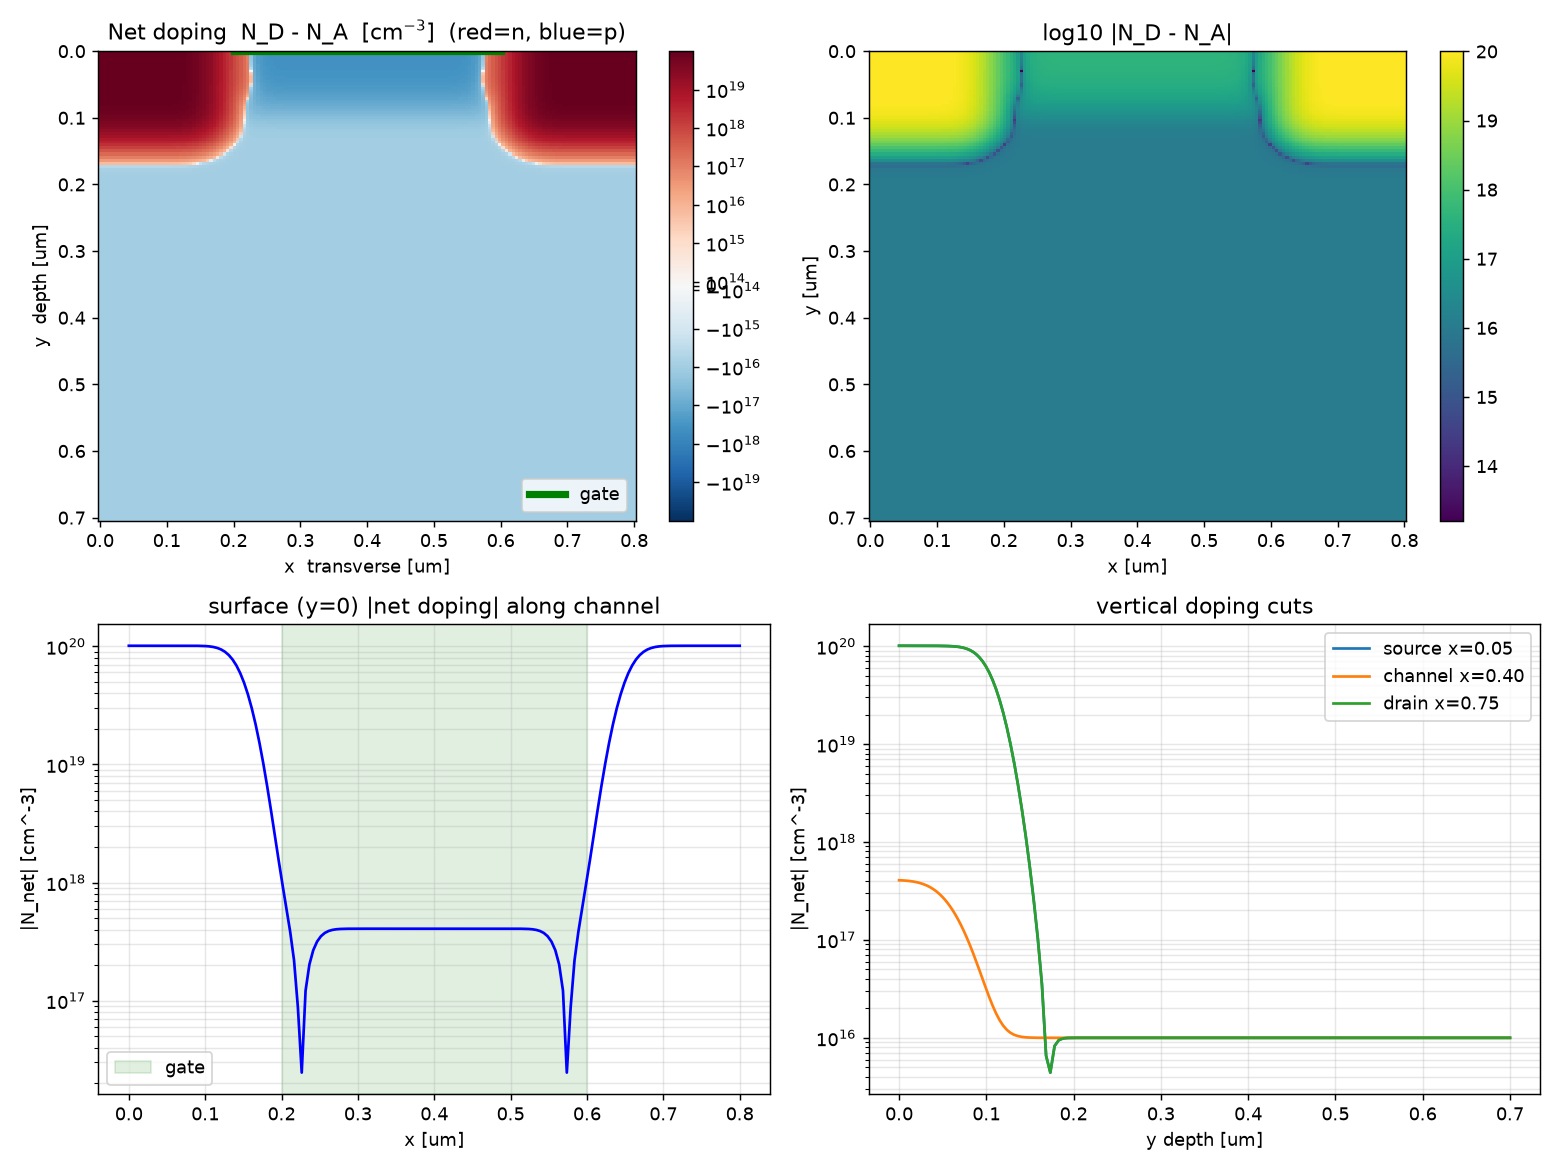
\includegraphics[width=\linewidth]{../figures/device_doping.png}
\caption{Reconstructed 0.35-\si{\micro\meter} LDD NMOS, $x_j=0.170\,\si{\micro\meter}$.}
\end{figure}

\section{Benchmarks, bulk validation, threshold voltage}\label{sec:bench}
\begin{table}[h]\centering\small
\caption{Foundation checks at $T=\SI{300}{K}$. \fix{m5} row classes corrected.}\label{tab:bench}
\begin{tabular}{p{5.4cm}r r p{3.3cm}}
\toprule
Quantity & Expected & Computed & Note\\
\midrule
\multicolumn{4}{l}{\emph{(A) Analytic benchmarks (independent)}}\\
$N_c$ nonparabolic (converged) & $2.86\times10^{19}$ & $2.857\times10^{19}$ & 0.1\%\\
$N_c$ parabolic: code vs.\ closed form & $2.726\times10^{19}$ & $2.723\times10^{19}$ & prefactor 0.09\%\\
$v(0.1)/v(1.0)$~eV [cm/s] & --- & $3.09/6.42\times10^{7}$ & auditor-reproduced\\
$V_{bi}$ [V] & $0.933$ & $0.933$ & $V_t\ln(N_DN_A/n_i^2)$\\
n$^+$ contact potential [V] & $0.586$ & $0.586$ & $V_t\ln(N_D/n_i)$\\
bulk $T_e(0)$ [K] & $309.7$ & $311$ & $\to$309.7 as $\Delta\eps\to0$\\
$T_e(\SI{300}{kV/cm})$ vs.\ $\eps_{max}$ & invariant & $3392.4$ & K; $\eps_{max}{=}3.02/4/5$ identical\\
\midrule
\multicolumn{4}{l}{\emph{(B) Construction targets (built-to)}}\\
metallurgical $x_j$ [\si{\micro\meter}] & $0.17$ & $0.170$ & retuned\\
\midrule
\multicolumn{4}{l}{\emph{(C) Method / qualitative sanity}}\\
Newton convergence & quadratic & quadratic & to $10^{-11}$, 6 steps\\
optical op.\ detailed balance / $E{=}0$ Maxwellian & $0$ & $2\!\times\!10^{-5}/3\!\times\!10^{-4}$ & null / max dev.\\
depletion width abrupt vs.\ graded [\si{\micro\meter}] & $0.347$ & $0.269$ & graded narrower (not equality)\\
bulk $T_e$ vs.\ field (0/100/300 kV/cm) [K] & monotone$\uparrow$ & 311/1478/3392 & heating\\
\bottomrule
\end{tabular}
\end{table}

\paragraph{Threshold voltage --- measured trend \fix{m3}.} Both electrostatic offsets are
fixed inputs and $V_{th}$ is \emph{derived} by max-$g_m$ linear extrapolation
($V_{ds}=\SI{0.1}{V}$). Measured: $V_{th}=\SI{1.64}{V}$ at $N_A=\SI{4e17}{cm^{-3}}$ and
$V_{th}=\SI{1.03}{V}$ at $N_A=\SI{1.2e17}{cm^{-3}}$. Both are \emph{too high}; the Rev.~3
guess that $N_A\!\sim\!\SI{1.2e17}{}$ reaches $V_{th}\approx\SI{0.6}{V}$ is \textbf{refuted}
by this measurement (it gives \SI{1.03}{V}). A paper-typical $V_{th}\approx0.5$--\SI{0.7}{V}
(inferred from the paper's Fig.~8b conducting at $V_{gs}=2$--\SI{3}{V}) will require a lower
implant ($N_A\!\lesssim\!\SI{6e16}{}$) and/or a gate-offset adjustment --- to be demonstrated
in the Part~II recalibration, not asserted here.

\paragraph{Drift-diffusion current.} With the extracted $V_{th}=\SI{1.64}{V}$
($N_A=\SI{4e17}{}$ device), overdrive $\SI{1.36}{V}$ gives long-channel
$\SI{0.28}{mA/\micro\meter}$ vs.\ DD $\SI{0.25}{mA/\micro\meter}$ (auditor-confirmed
\SI{0.285}{}); $\sim\!14\%$, the residual from velocity saturation.

\begin{figure}[h]\centering
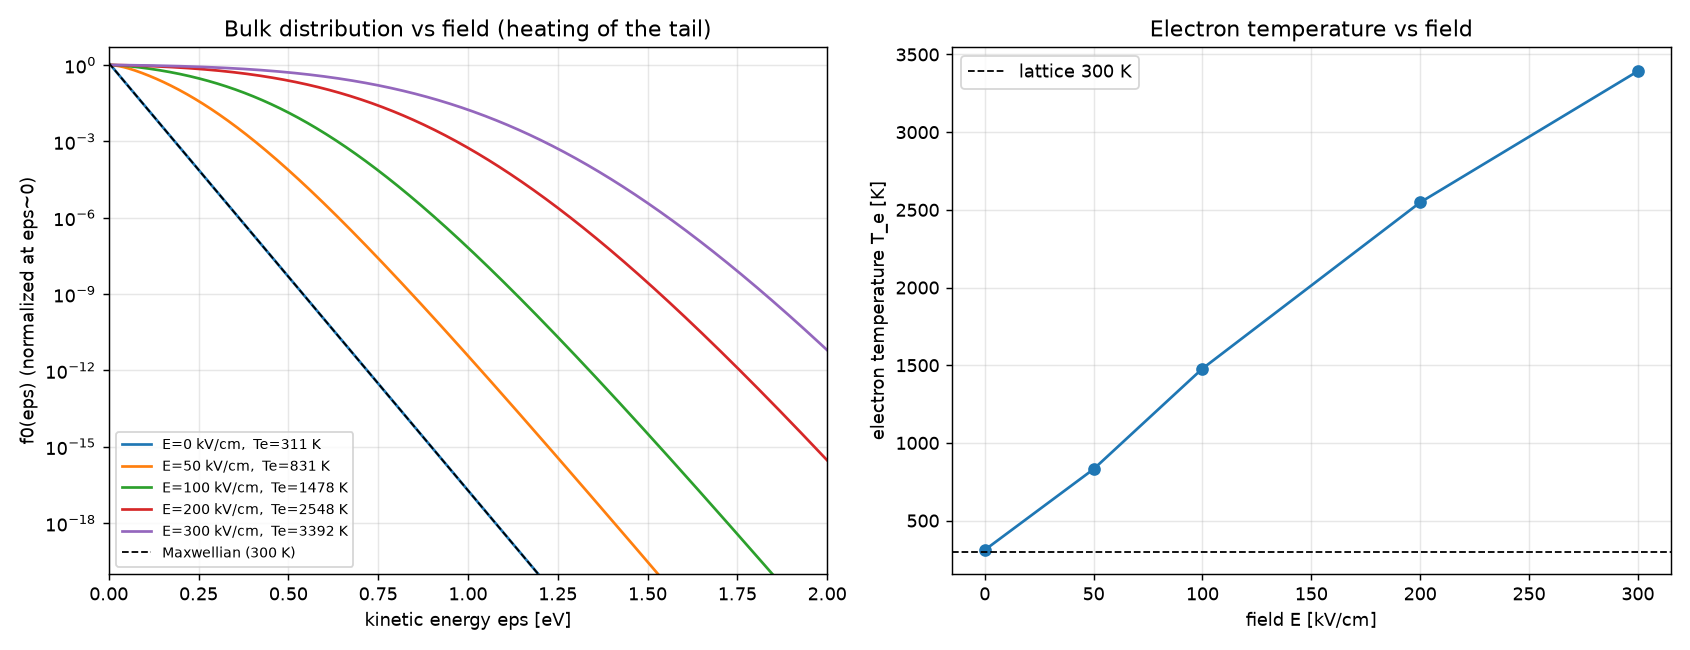
\includegraphics[width=0.82\linewidth]{../figures/she_bulk_validation.png}
\caption{Bulk validation (acoustic operator; absorbing $\eps_{max}$): zero field reproduces
the Maxwellian ($T_e=311\to309.7$~K), tail heats monotonically, and $T_e$ is
$\eps_{max}$-invariant. \emph{Bulk-prototype} validation; 2-D production scattering pending.}
\end{figure}

\section{Status}
\begin{center}\small
\begin{tabular}{clc}
\toprule
Phase & Component & Status\\
\midrule
P1 & Derivation (Rev.\ 4, thrice-audited) & \textcolor{green!60!black}{\textbf{documented}}\\
P2--P4 & Device, Poisson, DD, bands & \textcolor{blue!70!black}{\textbf{sanity-checked}}\\
P5 & First-order SHE core ($(\vecr,H)$) & in progress\\
P6 & Scattering: bulk prototype / 2-D production & \textcolor{blue!70!black}{prototype} / pending\\
P7--P9 & Impact ionization, self-consistent loop, Figs.~2--8 & pending\\
\bottomrule
\end{tabular}
\end{center}
\emph{Open device issue:} $V_{th}$ recalibration (\S\ref{sec:bench}) before the 2-D operating
point is finalized.

\appendix
\section{Numerical and model specifications}\label{sec:specs}
\textbf{Constants:} $T=\SI{300}{K}$, $V_t=\SI{25.85}{mV}$, $n_i=\SI{1.45e10}{cm^{-3}}$,
Boltzmann, $\epsilon_{si}=11.7$, $\epsilon_{ox}=3.9$, $m^*=0.32m_0$, $g_v=6$, $\alpha=
\SI{0.5}{eV^{-1}}$, $v_s=\SI{9.04e3}{m/s}$. \textbf{Doping (erfc), \si{\micro\meter}:}
$N_D=10^{20}[L(x;0.15)+R(x;0.65)]D(y;0.105)+10^{18}[L(x;0.22)+R(x;0.58)]D(y;0.06)$,
$L(x;e)=\tfrac12\mathrm{erfc}(\tfrac{x-e}{0.028})$, $R(x;e)=\tfrac12\mathrm{erfc}
(\tfrac{e-x}{0.028})$, $D(y;x_j)=\tfrac12\mathrm{erfc}(\tfrac{y-x_j}{0.025})$; $N_A=10^{16}+
N_A^{ch}\cdot\tfrac12[\mathrm{erfc}(\tfrac{x-0.62}{0.028})-\mathrm{erfc}(\tfrac{x-0.18}
{0.028})]D(y;0.06)$, $N_A^{ch}=\SI{4e17}{}$ (or $\SI{1.2e17}{}$, \S\ref{sec:bench}). Gate
$x\in[0.20,0.60]$; source $x\le0.15$, drain $x\ge0.65$ (top); body = bottom.
\textbf{Mesh:} tensor, surface-refined $y\propto s^{1.8}$; $N_x{\times}N_y=90{\times}80$
(Poisson), $80{\times}70$ (DD), $56{\times}48$ ($V_{th}$). \textbf{Bulk $\eps$-grid:} uniform
$\Delta\eps=\SI{2.5}{meV}$, $[0,3.02]$~eV. \textbf{Production $H$-grid \fix{m3}:} a
\emph{fixed} global grid (not regenerated during the Gummel loop --- avoids conservative
$f_0$ remapping), $\Delta H=\SI{2.5}{meV}$ so $E_{op}/\Delta H=20$ is an \emph{integer} (the
optical operator connects $H\!\leftrightarrow\!H\pm20$ nodes with no interpolation), range
from the a-priori bias envelope $[-q\phi_{max},\,\eps_{max}-q\phi_{min}]$ over all bias
points; $\eps=0$ reflecting, $\eps_{max}$ absorbing (\S\ref{sec:bc}). \textbf{Poisson BCs:}
ohmic Dirichlet $\phi=V+V_t\,\mathrm{asinh}(N_{net}/2n_i)$; gate oxide Robin
$T_{ox}=\epsilon_{ox}\epsilon_0\Delta x_i/t_{ox}$ ($t_{ox}=\SI{9.6}{nm}$) to node
$V_g-\Phi_{gate}$, $\Phi_{gate}=\SI{0.30}{V}$; Neumann else. Newton clip \SI{0.5}{V}, tol
\SI{e-8}{V}. \textbf{Continuity:} SG $J_{n,a\to b}=\tfrac{q\mu_nV_t}{h}[B(\Delta)n_b-B(-\Delta)
n_a]$; ohmic $n=\tfrac12(N_{net}+\sqrt{N_{net}^2+4n_i^2})$, $p=n_i^2/n$. \textbf{Mobility:}
Caughey--Thomas ($n$: $68.5/1414/9.2{\times}10^{16}/0.711$; $p$: $44.9/470.5/2.23{\times}
10^{17}/0.719$), $v_{sat}^n=\SI{1.07e7}{},\beta_n{=}2$; $v_{sat}^p=\SI{8.37e6}{},\beta_p{=}1$
[cm/s]. \textbf{SRH} $\tau_{n,p}=\SI{e-7}{s}$. \textbf{Gummel} tol \SI{e-5}{V}.
\textbf{Optical:} $c_{op}=\SI{4.69e-34}{J\,m^3/s}$ ($\tau_{op}^{ref}=\SI{e-13}{s}$),
$\tau_1=\SI{e-14}{s}/(\sqrt{\gamma}\gamma')$. \textbf{Acoustic:} $\tau_{ac}=\tau_1$,
$A=4m^*v_s^2\eps/\tau_{ac}$ (\S\ref{sec:acderiv}). \textbf{Contact current:} $\sum$ SG fluxes
into drain nodes, per \si{\micro\meter}. \textbf{SHE contact \fix{B(new)}:}
$f_0(\eps)=n_{contact}\,e^{-\eps/k_BT}/\!\int Z(\eps)e^{-\eps/k_BT}d\eps$ (\emph{no} $Z^{-1}$;
gives $n=\int Zf_0\,d\eps=n_{contact}$).

\section{Code and parameter provenance}\label{sec:provenance}
Git commit \texttt{e71677b}; Python 3.13.14, NumPy 2.5.1, SciPy 1.18.0. Modules:
\texttt{constants, device, poisson, dd, bands, scattering, she\_bulk, diagnostics,
vth\_extract}. Figures/benchmarks regenerated by running the corresponding module.

\begin{thebibliography}{9}\small
\bibitem{liang} W.~Liang \emph{et al.}, \emph{IEEE Trans.\ Electron Devices} \textbf{44}(2),
257--267, 1997.
\bibitem{fiegna} C.~Fiegna, E.~Sangiorgi, \emph{IEEE TED} \textbf{40}, 619, 1993.
\bibitem{brunetti} R.~Brunetti \emph{et al.}, \emph{Solid-State Electron.} \textbf{32}, 1663,
1989.
\bibitem{gnudi} A.~Gnudi \emph{et al.}, \emph{Solid-State Electron.} \textbf{36}, 575, 1993.
\bibitem{hennacy} K.~A.~Hennacy \emph{et al.}, \emph{Solid-State Electron.} \textbf{38}, 1489,
1995.
\bibitem{wu} Y.-J.~Wu, N.~Goldsman, \emph{J.\ Appl.\ Phys.} \textbf{78}, 1995.
\bibitem{khalil} N.~Khalil \emph{et al.}, \emph{Symp.\ VLSI Technol.}, 131, 1994.
\bibitem{sg} D.~L.~Scharfetter, H.~K.~Gummel, \emph{IEEE TED} \textbf{ED-16}, 64, 1969.
\bibitem{landsberg} P.~T.~Landsberg, ``Impact ionization and Auger recombination in bands,''
\emph{Solid State Commun.} \textbf{10}(6), 479--482, 1972.
\bibitem{caughey} D.~M.~Caughey, R.~E.~Thomas, \emph{Proc.\ IEEE} \textbf{55}, 2192, 1967.
\bibitem{jungemann} C.~Jungemann, B.~Meinerzhagen, \emph{Hierarchical Device Simulation}.
Springer, 2003.
\end{thebibliography}

\end{document}
